% Following magic comments allow for compilation of root file
% !TEX root = ../../../../temp_manuscript.tex

\chapter{Introduction}

When genetic changes occur during the production of new cells, the cells might start growing uncontrollably, this uncontrollable growth of new cells is commonly known as cancer. When these cancerous cells clump together, the single mass that they form is called a tumour.
Tumours can originate from and occur in almost every anatomical location, and the tumour location is not always the same as the location from which the cancerous cells originated.
When the tumour appears in the same anatomical location as the anatomical origin of the cells, the tumour is called a primary tumour.
Thus, primary brain tumours are tumours that are located in the brain and which are formed by cells that mutated from (healthy) brain cells.
Primary brain tumours are initially classified by the type of cells from which the tumour originated.
Thus many different categories of primary brain tumours exist, with gliomas being the most prevalent type \autocite{leece2017indicence}.
Gliomas originate from glial cells, which play a supporting role in the central nervous system and are the most abundant cell type in the brain \autocite{jakel2017glial}.

Although gliomas have a low incidence compared to other cancers, around \per{1.71} globally \autocite{leece2017indicence}, they are quite lethal with a median survival of around ten months \autocite{hess2004gliomaincidence}.
Historically gliomas were categorized based solely on their histological appearance, the appearance of the tumour cells under a microscope, and were classified as astrocytoma, oligoastrocytoma, oligodendroglioma or glioblastoma depending on the type of glial cells that were visible in the tumour tissue. The gliomas were also assigned grade, grade II, III, or IV, to indicate the aggressiveness of the tumour.  Astrocytoma, oligoastrocytoma, and oligodendroglioma are often grade II or grade III glioma, whereas glioblastoma are often grade IV.

Not only is this histological categorization and grading of the tumours very observer-dependent, it has also been found that within the different grades, but large differences between patient survival also exist. Grade III and grade IV glioma are often grouped and referred to as \gls{HGG}, whereas grade II glioma are referred to as \gls{LGG}. However, some grade III glioma show survival that is much more similar to grade II glioma than to grade IV glioma. It was found that this difference can be explained by the genetic mutations present within the tumour \autocite{eckel2015gliomagroups}.
Therefore, in 2016 the \gls{WHO} updated their categorization of glioma to include these molecular features \cite{louis20162016} and depend less on the histology alone.
This update has lead to better patient stratification and a more objective categorization of the glioma since the genetic analysis is less observer-dependent than the histological analysis. For the histological appearance, only the difference between glioblastoma and astrocytoma, oligoastrocytoma, and oligodendroglioma is now relevant. The difference between astrocytoma, oligoastrocytoma, and oligodendroglioma is now dictated by the genetic features of the tumour.

\begin{figure}[hbt]
    \resizebox{0.8\textwidth}{!}{\subimport{Figures/}{WHO_2016_flowchart.pgf}}
    \centering
    \caption{The WHO 2016 categorizaton of glioma.}\label{fig:intro_glioma_categorization}
\end{figure}


The two most important genetic markers are the \gls{IDH} mutation and \acl{1p19qcotion} which now, in addition to the histological appearance, dictate the categorization of glioma as can be seen in \cref{fig:intro_glioma_categorization}.  Within the grade II and grade III glioma, the following categories now exist:

\begin{itemize}
    \item Diffuse astrocytoma, \gls{IDH} wildtype
    \item Diffuse astrocytoma, \gls{IDH} mutated
    \item Oligodendroglioma,\gls{IDH} mutated and 1p/19q codeleted
\end{itemize}

No category exists for 1p/19q codeleted, \gls{IDH} wildtype glioma since it has been found that all 1p19q codeleted tumors are also IDH mutated \autocite{labussi20101p19qcodeletedIDH}. The oligodendroglioma group has the best prognosis in these group, with the diffuse astrocytoma IDH wildtype showing the worst prognosis. Due to the aggressiveness off IDH wildtype astrocytoma, it is even suggested that these are actually misclassified glioblastoma.

For the \gls{HGG}, the WHO 2016 guidelines do not provide a subclassification.
However, it has been found that \gls{MGMT} methylation is an important molecular marker, where patients with \gls{MGMT} methylation survive longer \autocite{martinez2007MGMT, gessler2018MGMT}.
Futhermore in \gls{HGG} the \gls{IDH} mutation status is also an important marker.

Not only is the survival of patients whose tumors contain these molecular features longer, tumors also respond differently based on the genetic alterations.
For example \gls{IDH} mutated glioma respond better to radiotherapy \autocite{juratli2015IDHtreatment}, whereas the 1p19q co-deletion status and MGMT methylation status might be predictors of the sensitivity to chemotherapy \autocite{idbaih2007markersresponse}.
Thus, it is important to know the genetic subtype of the glioma, both for the prognosis of the patient as well as for the treatment plan.

In current clinical practice, the genetic markers are determined either from a biopsy, where a small piece of the tumor is removed for analysis, or from the resected tumor, when the whole tumor (or as much as possible) is removed as part of the treatment.
In both cases an intrusive operation is needed in order to obtain the required tumor tissue.
Therefore, it would be beneficial if the molecular status of a glioma could be known without the need for a biopsy or resection.
Not only does this obviate the need for an intrusive operation, it also provides the information earlier in the treatment process which, especially in the case of the resection, might influence the decision on the treatment.
Therefore, a focus on radiological imaging and specifically \gls{MRI} has been placed to see whether it is possible to identify the different tumor categories.

\gls{MRI} uses the property of the water molecules of tissue to form an image, by manipulating these properties, different tissue characteristics can be imaged.
These concept is often used in clinical care, mainly to distinguish healthy tissue from diseased tissue.
Shortly after the first introduction of \gls{MRI}, it was proposed that the method could be used to identify tumors \autocite{damadian1971tumor}.
After some improvements, the technique was first applied to the brain in 1980 \autocite{holland1980brain}, and in the same year MRI has first been used to investigate a possible tumor in the brain, shown in \cref{fig:intro_MR_first} \autocite{hawkes1980NMRbrain}.
Since then quality of \gls{MRI} scans has vastly increased, and different \gls{MRI} techniques have been developed that image different tissue characteristics.
\cref{fig:intro_MR_modern} shows a modern \gls{MR} image of a brain tumor.
Here the tumor can clearly be seen in the patients brain, and therefore \gls{MRI} is now the standard-of-care for brain tumor diagnosis and treatment decisions.

\begin{figure}[hbt]
    \centering
    \begin{subfigure}[b]{0.45\textwidth}
        \centering
        \includegraphics[width=\textwidth]{example-image-a}
        \caption{First scan of a human glioma}\label{fig:intro_MR_first}
    \end{subfigure}
    \begin{subfigure}[b]{0.45\textwidth}
        \centering
        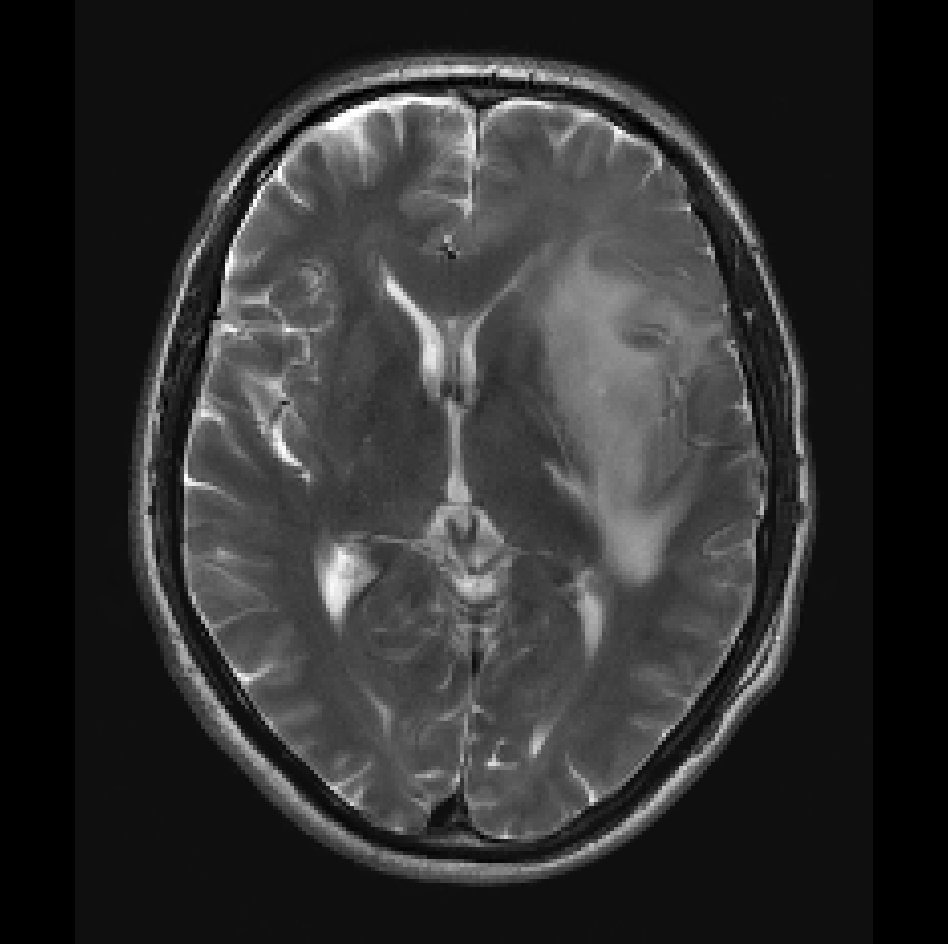
\includegraphics[width=\textwidth]{Figures/T2_LGG.png}
        \caption{Modern glioma scan}\label{fig:intro_MR_modern}
    \end{subfigure}
    \caption{\acrshort{MRI} scan of a glioma from 1980 and a recent \acrshort{MR} scan, showing the large improvement over time. On the modern scan the glioma can easily be identified}\label{fig:intro_MR_comparison}
\end{figure}

\gls{MRI} scans are already routinely being used to get a first indication of the aggressiveness of the tumor, mainly for the evaluation of the grade \autocite{upadhyay2011MRIevaluation}.
In recent years it has been shown that the certain imaging features can predict the status of the genetic markers of a tumor \autocite{patel2017mismatch, smits2016imaging}.
This has increased the interest for methods that can predict the genetic status of the tumor from the radiological images.
However, although research shows the existence of certain imaging characteristics that correlate with the gentic status, called biomarkers, the implementation of these methods in the clinical practice has still been limited.
This is due to a number of reasons.
Firstly, \gls{MRI} is a qualitative and not a quantitative measurement.
Thus it is hard to define a proper measurement value from an \gls{MR} scan, and thus to define a robust method that can easily be broadly applied.
Secondly, most biomarkers are rather simple; looking at a single point in the tumor or only considering the 2D measurements of a tumor.
Methods are kept simple so that they can easily be used by the clinician and do not require complicated, time-consuming measurement.
However, this limits the amount of information that such a method can take into account, thus pressing on the performance of these methods.
Lastly, the expertise of a clinician, the difference between \gls{MR} scans and the relatively poorly defined measurements cause a large inter- and intra-observer variability in the measurements.
This makes it difficult to broadly apply a method, causes a drop in performance and results in the patient treatment being dependent on the treating physician.
Thus, a method that would be more objective and consistent, that can take into account complex relationships of the image, while not being too complex and time-consuming for the clinician to use is needed.

This demand was met by the field of machine learning.
Machine learning leverages large amounts of data to find common patterns and uses these patterns to classify the data.
In the biomedical imaging field machine learning methods are often been used to classify images as disease vs healthy or to classify the state of a disease.
This area of research is called \say{radiomics}, where a subfield which focuses on predicting the genetic markers based on imaging is called \say{radiogenomics}.
In the (neuro-)oncology fields radiogenomics quickly gained in popularity, largely due to the WHO 2016 redefinition which was now based on the genomic status.
An in-depth introduction of machine learning, radiomics and the different methods is given in \cref{chap:radiomics}.

Using machine learning and other automated methods allows for a larger availability of information, which a clinician can use for the diagnosis and treatment decision of a patient.
Therefore, in this research we investigate different methods with which we can gain more insight into gliomas from MR imaging. This thesis has three main goals:
\begin{itemize}
\item Add to the knowledge of biomarkers of glioma, which experts can use to evaluate new patients
\item Automate analysis of glioma MR imaging to provide information about the clinical characteristics of the tumor
\item Provide automated tools and structured data to make glioma MR research available to a broader public more quickly.
\end{itemize}

The thesis is structured as follows:

In \cref{chap:radiomics} introduce the concept of machine learning and radiomics and detail the different terms used, as well the proper way to carry out such experiments.

In \cref{chap:LGGLocation} and \cref{chap:HGGLocation} there is a focus on the relationship between the molecular status of glioma and their location in the brain.
Here we investigate whether from the location of the tumor it is possible to say something about the (likely) molecular status, and thus whether the location of the glioma is a biomarker.

In \cref{chap:LGG1p19q} I use a machine learning method to predict the 1p/19q co-deletion status of low grade glioma.
Here we show that it is possible to automate this task, and that our method also extends to a different independent set.
We also present some biomarkers that our method found and showed that these have similarities with known biomarkers from literature.

In \cref{chap:discussion} I discuss the results from all the previous chapter and explore the possibilities for future directions.
